% Change "draft" to "final" when you're done.
\documentclass[12pt,letterpaper,oneside]{report}

\usepackage[top=1in,left=1.5in,right=1in,bottom=1in]{geometry}

\usepackage{fontspec,lipsum}
\usepackage{mathpazo}
\defaultfontfeatures{Ligatures=TeX}
\usepackage[small,sf,bf]{titlesec}

\usepackage{xltxtra}
\usepackage{xunicode}

\usepackage{subcaption}
\usepackage{graphicx}
\usepackage{rotating}

\graphicspath{{images/}}

%\DisemulatePackage{setspace}
\usepackage{setspace}
%\onehalfspacing
\doublespacing

\usepackage{titling}

\usepackage{unicode-math}
\usepackage{amsmath}
\usepackage{amsthm}

\usepackage{algorithm}
\usepackage{algorithmic}

%\usepackage{minted}
\usepackage{tikz}

\usepackage{booktabs}

\usepackage{nag}

\input tikz
\usetikzlibrary{fit}

\setmainfont[
	Numbers=OldStyle,
	Kerning=Uppercase,
	SizeFeatures={
		{Size={8-10}, Font=* Caption},
		{Size={10.01-}, Font=*}
	}]{Garamond Premier Pro}
\setsansfont{Futura Std}
\setmathfont{STIXGeneral}
\setmonofont{Consolas}

\pagenumbering{roman}

\newcommand{\thesistitle}[8]{
	\title{#1}
	\author{#2}

	\begin{titlepage}
		\centering
		\vspace{2cm}
			{\huge\sc #1}\\[1cm]

			by\\[1cm]

			{\Large #2}\\[2cm]

			\singlespacing{A Thesis Submitted in Partial Fulfillment\\of the Requirements for the Degree of}\\[1cm]

			#3\\[0.5cm]

			in\\[0.5cm]

			Faculty of #4\\[0.5cm]

			#5\\[1.5cm]

			University of Ontario Institute of Technology\\[1.5cm]

			Supervisor:  #6\\[1.5cm]

			#7 #8\\[3cm]

			Copyright \copyright\ #2 #8
	\end{titlepage}}

\theoremstyle{definition}
\newtheorem{defn}{Definition}

\begin{document}
	\thesistitle{Molly}{Richard Drake}{Masters of Science}{Science}{Computer Science}{Dr. Ken Q. Pu}{September}{2012}

	\begin{abstract}
		\lipsum[2]
	\end{abstract}

%	\begin{acknowledgements}
%		\lipsum[2]
%	\end{acknowledgements}

	\chapter*{Preface}
		\section*{Background and Motivation}
			The introduction of keyword search has revolutionized how we find information.  Over the years, numerous techniques have been developed which make searching through large amounts of information for one or more keywords extremely fast.  With the advent of faster computer hardware, we are able to not only search through small attributes of a document (eg. Title, synopsis, etc.) but rather the entirety of the document itself.
		
			An example of an early system which utilized keyword search would be a library catalogue.  Such a system would allow a user to search, by keyword, for the title of a book, manuscript, etc.  The results would show item titles matching the keyword(s), as well as other information such as whether or not the item is in circulation, as well as where it is located within the library.  This information would come from a relational database.
		
			With the rise of the World Wide Web, much information was placed online.  This information would be easy to access if one knew how to locate it.  Unfortunately, over time, so much information existed on the World Wide Web that it became difficult to keep track of it all.  There was a need to index all of this information and make it accessible.  This need was filled by a Web search engine.
		
			Initial Web search engines comprised of simple scripts that gathered listings of files on FTP servers; they were essentially link farms.  A few short years later, the first full-text (keyword) search engine, WebCrawler, was released.
		
			While full-text search engines provided an excellent means for locating information, as the Web grew larger, the volume of noise also grew larger.  In addition, every Web page could be structured in a different way; the Web was largely a collection of unstructured documents.  That is, there were few obvious links between them.
		
			Search engines such as Google attempted to solve this problem by introducing new algorithms, such as PageRank, to rank Web pages on both the relevance of their content as well as their reputation.  The idea was if a page is linked to often, it is considered to be more authoritative on a subject than a page with fewer links.  This allowed the relevance of a page to be computed based on not only its contents, but its artificial importance.
		
			Molly attempts to avoid some of the issues plaguing search engines.  It deals primarily with structured, filtered data.  This allows us to provide results with less noise.  In addition, the fact that it deals with structured data means links between documents are explicitly stated.  Rather than inferring a link between documents based on hyperlinks, we know when two documents are linked together.
		
			This thesis provides an overview of the Molly system.
		
		\section*{Outline}
			Changed.

	\tableofcontents

	\listoftables
	\listoffigures
	\listofalgorithms

	\clearpage
	\pagenumbering{arabic}

	\chapter{Literature Review}
	
	\chapter{Theoretical}
		The problem of efficiently searching through a graph is the subject of countless articles and journal papers.  Numerous algorithms have been proposed to perform graph search in an efficient manner.  Many of these algorithms build upon their predecessors, making assumptions and changing aspects to better suit a particular problem area.
		
		The applications of efficient graph search algorithms are endless.  Algorithms such as Dijkstra's are used heavily in path finding, for example in a portable GPS unit.  A* Search is used in the area of computer vision to approximate the best path to take.  Companies such as Amazon make use of graph search algorithms in order to find related products for consumers to purchase.
		
		This thesis concentrates on building a system which can be utilized in order to discover related information.  The system that was built is capable of finding not only related information from neighbouring nodes, but also the best path between two arbitrary nodes.
		
		Section \ref{sec:data-rep-and-notation} provides an overview of how the data is represented in the system.  It also defines notation to represent this data.  Section \ref{sec:database-abstraction} outlines how the relational database is related to the data in the system.  Section \ref{sec:data-corpus} provides an example data corpus which is utilized throughout this thesis.  It details the ``mycampus'' dataset.  Finally, Section \ref{sec:graph-search-algos} provides justification for the algorithm chosen to perform the graph search.  It discusses multiple different graph search algorithms, as well as why the one used in this thesis was chosen.
		
		\section{Data Representation \& Notation}
		\label{sec:data-rep-and-notation}
			The data from the database is represented in various data structures.  There are separate representations for each type of data:  values, entities, and entity groups.

				\subsubsection{Value}
					\begin{defn}
						A \textbf{Value} represents a single piece of information.  To avoid repetition, each value is unique.  That is, $\exists! v \in V$, where $v$ is a value in the set $V$ of all values.
					\end{defn}

				\subsubsection{Entity}
					\begin{defn}
						An \textbf{Entity} is a collection of attributes, $a_n$, each mapped to a single value, $v_n$.  An entity also includes additional information such as a unique identifier.

						\begin{figure}[!ht]
							\centering
							\[
								\begin{array}{ll}
									\mathrm{id} & T_n|v_{id} \\
									a_1 & v_1 \\
									a_2 & v_2 \\
									\vdots & \vdots \\
									a_n & v_n
								\end{array}
							\]
							\caption{The structure of an entity}
							\label{fig:entity-rep}
						\end{figure}

						Entities are analogous to rows in a database table.  Thus, the unique identifier is generated based on the table name, $T_n$, as well as unique key in the table, $v_{id}$.  The unique key identifies the row, and the table name identifies the table.  Together they uniquely identify the entity within the entire database.

						$\exists! e_{id} \in E$, where $E$ is the set of all entities.
					\end{defn}

				\subsubsection{Entity Group}
					\begin{defn}
						An \textbf{Entity Group} joins together two or more entities.  These entity groups can also have attributes, $a_n$, and values, $v_n$, associated with them much like entities.

						\begin{figure}[!ht]
							\centering
							\[
								\begin{array}{ll}
									e_L & \left[ e_1, e_2, \ldots, e_n \right] \\
									a_1 & v_1 \\
									a_2 & v_2 \\
									\vdots & \vdots \\
									a_n & v_n
								\end{array}
							\]
							\caption{The structure of an entity group}
							\label{fig:entity-group-rep}
						\end{figure}

						\begin{tikzpicture}[auto=left,every node/.style={circle}]
							\node (e1) at (1,1) {$e_1$};
							\node (e2) at (4,1)  {$e_2$};
							\node (e3) at (7,1)  {$e_3$};
							\node (e4) at (10,1) {$e_4$};
							\node (e5) at (13,1)  {$e_5$};

							\foreach \from/\to in {e1/e2,e2/e3,e3/e4,e4/e5}
								\draw (\from) -- (\to);
							
							\node (rect) [draw,dotted,fit=(e1) (e2) (e3)] {};
							\node[draw,dotted,fit=(e3) (e4) (e5)] {};

						\end{tikzpicture}
					\end{defn}
					
		\section{Relational Database Abstraction}
		\label{sec:database-abstraction}
		
		\section{Data Corpus}
		\label{sec:data-corpus}
			For illustrative purposes, the mycampus dataset will be used.  This data comes from UOIT's course registration system.
			
			There are several different entities which comprise the mycampus dataset:
			
			\begin{itemize}
				\item Courses
				\item Instructors
				\item Schedules
				\item Sections
				\item Teaches
			\end{itemize}
			
			The \textbf{Courses} entity represents a course.  A course has an individual code, along with a title and a description (See Table  \ref{tbl:courses-entity-schema}).  The code uniquely identifies the course.
			
			\begin{table}[!htp]
				\centering
				\begin{tabular}{lll}
					\toprule
					Column & Type & Description \\
					\midrule
					code & VARCHAR & Unique course code \\
					title & VARCHAR & Title of the course \\
					description & TEXT & A brief description \\
					\bottomrule
				\end{tabular}
				\caption{Courses entity schema}
				\label{tbl:courses-entity-schema}
			\end{table}
			
			The \textbf{Instructors} entity represents an individual instructor.  Each instructor has a unique identifier, as well as a name (See Table \ref{tbl:instructors-entity-schema}).  An instructor can be a Professor, Lecturer, Sessional Instructor, or Teaching Assistant.
			
			\begin{table}[!htp]
				\centering
				\begin{tabular}{lll}
					\toprule
					Column & Type & Description \\
					\midrule
					id & INT & Unique identifier \\
					name & VARCHAR & The instructor's name \\
					\bottomrule
				\end{tabular}
				\caption{Instructors entity schema}
				\label{tbl:instructors-entity-schema}
			\end{table}
			
			The \textbf{Sections} entity represents a section of a course.  Courses may have many sections.  For example, one section could be a lecture, while another is a lab.  Some courses may have over a dozen sections, depending on the associated term.
			
			Each section contains a unique identifier, capacity information (students enrolled, spots open, etc.), when registration is open for the section, how many credits it is worth, what level (eg. undergraduate or graduate), and what year the section is offered in (See Table \ref{tbl:sections-entity-schema}).
			
			\begin{table}[!htp]
				\centering
				\begin{tabular}{lll}
					\toprule
					Column & Type & Description \\
					\midrule
					id & INT & Unique identifier \\
					actual & INT & Number of people enrolled in the course \\
					campus & VARCHAR & String uniquely identifying the campus \\
					capacity & INT & Maximum number of people that may be enrolled in the section \\
					credits & FLOAT & Number of credits awarded upon successful completion \\
					levels & VARCHAR & The level of the course (eg. undergraduate, graduate, etc.) \\
					registration\_start & DATE & Date registration for the section opens \\
					registration\_end & DATE & Date registration for the section ends \\
					semester & VARCHAR & String that uniquely identifies the semester \\
					sec\_code & INT & Unique section code (called a CRN) \\
					sec\_number & INT & Sequential number identifying the number of the section \\
					year & INT & The year the section is offered in \\
					\bottomrule
				\end{tabular}
				\caption{Sections entity schema}
				\label{tbl:sections-entity-schema}
			\end{table}
			
			The \textbf{Schedules} entity represents a scheduled meeting of a section.  A section may have many schedules.  For example, a lecture section may meet twice a week.
			
			Each schedule has a unique identifier, a date range in which the schedule is active, the time of the schedule, the type, location, and the day which the class takes place (See Table \ref{tbl:schedules-entity-schema}).
			
			\begin{table}[!htp]
				\centering
				\begin{tabular}{lll}
					\toprule
					Column & Type & Description \\
					\midrule
					id & INT & Unique identifier \\
					date\_start & DATE & First day of class \\
					date\_end & DATE & Last day of class \\
					day & VARCHAR & Single character representing the day of the week \\
					schedtype & VARCHAR & Lecture, tutorial, lab, etc. \\
					hour\_start & INT & Hour the class starts at \\
					hour\_end & INT & Hour the class ends at \\
					min\_start & INT & Minute the class starts at \\
					min\_end & INT & Minute the class ends at \\
					classtype & VARCHAR & The type of class \\
					location & VARCHAR & Unique location name where class is held \\
					\bottomrule
				\end{tabular}
				\caption{Schedules entity schema}
				\label{tbl:schedules-entity-schema}
			\end{table}
			
			A \textbf{Teaches} entity is used to link together an instructor and a schedule.  Each link has a unique identifier along with the instructor's position (eg. Teaching Assistant, Lecturer, etc.) (See Table \ref{tbl:teaches-entity-schema}).
			
			\begin{table}[!htp]
				\centering
				\begin{tabular}{lll}
					\toprule
					Column & Type & Description \\
					\midrule
					id & INT & Unique identifier \\
					position & VARCHAR & Position of the Instructor with regard to a Schedule \\
					\bottomrule
				\end{tabular}
				\caption{Teaches entity schema}
				\label{tbl:teaches-entity-schema}
			\end{table}
		
		\section{Graph Search Algorithms}
		\label{sec:graph-search-algos}
			Careful consideration was given to which graph search algorithm was to be used.  Among the choices were:
			
			\begin{itemize}
				\item Breadth-First
				\item Bellman-Ford
				\item Dijkstra
				\item A*
			\end{itemize}
			
			The first choice, Breadth-First Search, is among the simplest of the algorithms.  It has the advantage of being simple to implement.  It can only handle fixed costs for travelling between nodes, which can be a disadvantage.
			
			Bellman-Ford is similar to BFS.  It has the ability to deal with variable cost.  This comes at the cost of increased difficulty in implementation.  When the cost between nodes is fixed, Bellman-Ford essentially becomes BFS.
			
			A greedy version of BFS is Dijkstra's Algorithm.  It utilizes a priority queue rather than a regular queue, allowing it to be faster.  As it is a greedy algorithm, Dijkstra's Algorithm may not return the optimal result.
			
			An extension to Dijkstra's is A* search.  Graph search spaces can be rather large.  A* attempts to prune the search space based on a heuristic.  A* is a natural choice to perform graph search in certain areas such as computer vision where an obvious heuristic exists.  It has a disadvantage of consuming large amounts of memory (though IDA* attempts to limit memory consumption).
			
			There are many more graph search algorithms.  The above were primarily considered as many of the other algorithms are simple extensions with different data structures.
			
			For this application, there is no obvious heuristic.  This eliminates A*.  There is also no obvious cost function.  This eliminiates Dijkstra's Algorithm.  Bellman-Ford is very similar to BFS with the added ability to deal with variable cost.  As the cost function is not obvious and thus constant, Bellman-Ford essentially reverts back to BFS.
			
			For these reasons, BFS was chosen as the graph search algorithm.  While the other candidates and others provide numerous advantages over BFS in many situations, this is not one of them.
	
	\chapter{Implementation}
		\section{Functional vs. Procedurial Programming of Algorithms}
			Key differences between FP and procedurial (for algorithms)
			
			\subsection{Functional Data Structures}
				Clojure immutable data structures, versioning (persistent data structures), STM vs. locking
			
		\section{Tunable Parameters}
			Tunable parameters
	
	\chapter{System Implementation}
		\section{Technology Selection}
			
			
			\subsection{Programming Language}
				Numerous programming languages were considered for the implementation.  Among them were:  Ruby, Python, and Clojure.  Each of the languages presented both pros and cons.  Ruby and Python are rather similar object oriented languages.  Clojure is a functional language.
				
				Ruby features a clean syntax and is very object oriented.  Its object model was inspired by that of Smalltalk.  It has a very active web development community and numerous web frameworks (eg. Rails, Sinatra, Padrino, etc.).  In contrast to Python, it features a lean core, instead choosing to depend on third party libraries.
				
				Python also features clean syntax and is object oriented.  It embraces a ``batteries included'' philosophy to its standard library, featuring libraries for everything from serial communications to importing/exporting CSV files.  It too has a strong web development community and numerous web frameworks (eg. Django, Flask, web2py, etc.).
				
				Python is used extensively by scientists.  As such, it has numerous plotting, computation, and simulation libraries.  Examples include Matplotlib, SciPy, NumPy, and NetworkX.
				
				Both of the above languages embrace functional programming elements.  Python has filter, reduce, and map.  Ruby's collections are also capable of performing filter (select), reduce (inject), and map.  They both lack an important aspect of functional programming:  immutable objects.
				
				Clojure is a purely functional language built on top of the JVM.  Like Python and Ruby, it is dynamically typed.  Unlike Python and Ruby, it is a Lisp dialect and as such features macros and code-as-data.
				
				As it runs on the JVM, Clojure allows us to utilize existing Java languages.  Using Java libraries through Python or Ruby requires using their respective native code interfaces to Java's JNI.  This process is typically automated through a tool such as SWIG.
				
				Clojure was chosen as the implementation language for a number of reasons.  First of all, as it is built on top of the JVM, it can utilize JDBC for database access.  It can also make use of several other useful libraries.  Secondly, its dynamic Lisp nature is a natural way of processing data.  Clojure allows us to model our data structures directly after the data.  In a language such as Python, one would need to make use of classes.
			
			\subsection{Relational Database}
			
			\subsection{Full-Text Search Database}
			
			\subsection{Web Stack}
		
		\section{Implementation Issues}
	
	\chapter{Performance \& Evaluation}
		\section{Methodology}
			Evaluating the performance of code is a difficult problem at best.  It is difficult to determine the impact on performance of various uncontrollable factors.  Virtual Machines add another layer of abstraction which introduces even more factors.
			
			As this project runs a top of the Java Virtual Machine (JVM), there are many factors to consider with regard to performance.  In addition to uncontrollable events such as garbage collection, the JVM's behaviour can differ based on the operating system (OS) it is running on.
			
			\subsection{Pitfalls of the Java Virtual Machine}
				
				\subsubsection{Timing Execution}
					There are two methods provided by the JVM for getting a precise time from the OS; \texttt{System.currentTimeMillis()} and \texttt{System.nanoTime()}.  The former returns the ``wall'' time.  It is possible for time to leap forward or backward using this method.  If daylight savings time occurs between calls to \texttt{System.currentTimeMillis()}, it can result in a negative time.
					
					The latter uses a variety of methods in order to obtain the precise time.  The method it uses depends on both the OS and the hardware itself.  Under Windows, \texttt{System.nanoTime()} makes use of the \texttt{QueryPerformanceCounter(QPC)} call.  This call may make use of the ``programmable-interval-timer (PIT), or the ACPI power management timer (PMT), or the CPU-level timestamp-counter (TSC).'' (https://blogs.oracle.com/dholmes/entry/inside\_the\_hotspot\_vm\_clocks)  Accessing the PIT and PMT is a slow operation.  Accessing the TSC is a very fast operation, but may result in varying numbers (http://lwn.net/Articles/209101/).
					
					Linux attempts to use the TSC when possible.  If it finds the values to be unreliable (eg. different cores vary too much), it makes use of the High Precision Event Timer (HPET) (http://lwn.net/Articles/209101/).
					
				The JVM's timing functions are one area where the JVM's behaviour differs based on the OS.  Different operating systems provide varying degrees of time resolution.  The speed at which the OS-level calls to these timing functions return can even differ.
				
			\subsubsection{Garbage Collection}
				
		
		\begin{figure}[!ht]
			\centering
			\includegraphics[scale=0.85]{1_hops}
			\caption{1 Hop}
			\label{fig:perf-1-hop}
		\end{figure}
		
		\begin{figure}[!ht]
			\centering
			\includegraphics[scale=0.85]{2_hops}
			\caption{2 Hops}
			\label{fig:perf-2-hops}
		\end{figure}
		
		\begin{figure}[!ht]
			\centering
			\includegraphics[scale=0.85]{3_hops}
			\caption{3 Hops}
			\label{fig:perf-3-hops}
		\end{figure}
		
		\begin{figure}[!ht]
			\centering
			\includegraphics[scale=0.85]{4_hops}
			\caption{4 Hops}
			\label{fig:perf-4-hops}
		\end{figure}
		
		\begin{figure}[!ht]
			\centering
			\includegraphics[scale=0.85]{5_hops}
			\caption{5 Hops}
			\label{fig:perf-5-hops}
		\end{figure}
		
		\begin{figure}[!ht]
			\centering
			\includegraphics[scale=0.85]{6_hops}
			\caption{6 Hops}
			\label{fig:perf-6-hops}
		\end{figure}
		
		\begin{figure}[!ht]
			\centering
			\includegraphics[scale=0.85]{7_hops}
			\caption{7 Hops}
			\label{fig:perf-7-hops}
		\end{figure}
		
		\begin{figure}[!ht]
			\centering
			\includegraphics[scale=0.85]{8_hops}
			\caption{8 Hops}
			\label{fig:perf-8-hops}
		\end{figure}
		
		\begin{figure}[!ht]
			\centering
			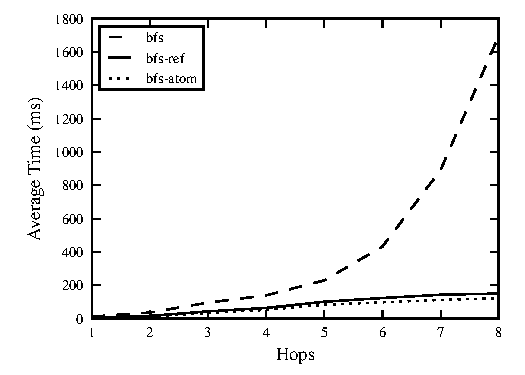
\includegraphics[scale=0.85]{growth}
			\caption{Comparison between single threaded and concurrent graph search}
			\label{fig:perf-growth}
		\end{figure}
		
%		\begin{sidewaysfigure}[!ht]
%			\subcaptionbox{1 Hop\label{fig:perf-1-hop}}[0.5\linewidth]{\includegraphics[scale=1.1]{../1_hops}}
%			\subcaptionbox{2 Hops\label{fig:perf-2-hops}}[0.5\linewidth]{\includegraphics[scale=1.1]{../2_hops}}
%			\subcaptionbox{3 Hops\label{fig:perf-3-hops}}[0.5\linewidth]{\includegraphics[scale=1.1]{../3_hops}}
%			\subcaptionbox{4 Hops\label{fig:perf-4-hops}}[0.5\linewidth]{\includegraphics[scale=1.1]{../4_hops}}
%			\caption{Results of 1-4 Hops}
%		\end{sidewaysfigure}
%		
%		\begin{sidewaysfigure}[!ht]
%			\subcaptionbox{5 Hops\label{fig:perf-5-hops}}[0.5\linewidth]{\includegraphics{../5_hops}}
%			\subcaptionbox{6 Hops\label{fig:perf-6-hops}}[0.5\linewidth]{\includegraphics{../6_hops}}
%			\subcaptionbox{7 Hops\label{fig:perf-7-hops}}[0.5\linewidth]{\includegraphics{../7_hops}}
%			\subcaptionbox{8 Hops\label{fig:perf-8-hops}}[0.5\linewidth]{\includegraphics{../8_hops}}
%			\caption{Results of 5-8 Hops}
%		\end{sidewaysfigure}
		
		Screenshots?
		Graphs
		Experiments
	
	\chapter{Conclusion}
	
\end{document}
